% Copyright (c) 2022 by Lars Spreng
% This work is licensed under the Creative Commons Attribution 4.0 International License.
% To view a copy of this license, visit http://creativecommons.org/licenses/by/4.0/ or send a letter to Creative Commons, PO Box 1866, Mountain View, CA 94042, USA.
%
%~~~~~~~~~~~~~~~~~~~~~~~~~~~~~~~~~~~~~~~~~~~~~~~~~~~~~~~~~~~~~~~~~~~~~~~~~~~~~~
% ICML 2026 short presentation (target length: 4:30-4:45).
% Paper: "Predictive Prefetching for Retrieval-Augmented Generation"
% Authors: Wuyang Zhang, Shichao Pei (University of Massachusetts Boston)
% Speaker notes for each slide live in the \note{...} blocks and are hidden
% in the exported PDF. Uncomment the \setbeameroption line below to see them.
%~~~~~~~~~~~~~~~~~~~~~~~~~~~~~~~~~~~~~~~~~~~~~~~~~~~~~~~~~~~~~~~~~~~~~~~~~~~~~~

\documentclass[
t,11pt,notheorems,hyperref={pdfauthor={Wuyang Zhang, Shichao Pei}}
]{beamer}


% Copyright (c) 2022 by Lars Spreng
% This work is licensed under the Creative Commons Attribution 4.0 International License. 
% To view a copy of this license, visit http://creativecommons.org/licenses/by/4.0/ or send a letter to Creative Commons, PO Box 1866, Mountain View, CA 94042, USA.

%~~~~~~~~~~~~~~~~~~~~~~~~~~~~~~~~~~~~~~~~~~~~~~~~~~~~~~~~~~~~~~~~~~~~~~~~~~~~~~
% Add your packages and commands to this file
%~~~~~~~~~~~~~~~~~~~~~~~~~~~~~~~~~~~~~~~~~~~~~~~~~~~~~~~~~~~~~~~~~~~~~~~~~~~~~~

%~~~~~~~~~~~~~~~~~~~~~~~~~~~~~~~~~~~~~~~~~~~~~~~~~~~~~~~~~~~~~~~~~~~~~~~~~~~~~~
% Fonts
% \RequirePackage{palatino} % for serif slides
% \usefonttheme{serif}
\RequirePackage[scaled]{helvet} % for sans-serif slides

\RequirePackage[utf8]{inputenc}
\RequirePackage[T1]{fontenc}


\usepackage{styles/elegantmacros}
\usefolder{styles}
\usetheme[style=gray]{elegant}

\newcommand{\makepart}[1]{ % For convenience
\part{#1} \frame{\partpage}
}

%~~~~~~~~~~~~~~~~~~~~~~~~~~~~~~~~~~~~~~~~~~~~~~~~~~~~~~~~~~~~~~~~~~~~~~~~~~~~~~

%~~~~~~~~~~~~~~~~~~~~~~~~~~~~~~~~~~~~~~~~~~~~~~~~~~~~~~~~~~~~~~~~~~~~~~~~~~~~~~
% Figures
\RequirePackage{booktabs}
\RequirePackage{colortbl}
\RequirePackage{ragged2e}
\RequirePackage{schemabloc}
%\RequirePackage{natbib}
\RequirePackage{caption}
\RequirePackage{subcaption}
\RequirePackage{tabularx}
\RequirePackage{array}
\RequirePackage{multirow}
\RequirePackage[%
  natbib=true, backend=biber,%
  style=apa, isbn=false,url=false,uniquename=false%, useprefix=true%
  ]{biblatex}
\addbibresource{references.bib}
\newcolumntype{Y}{>{\centering\arraybackslash}X}

%~~~~~~~~~~~~~~~~~~~~~~~~~~~~~~~~~~~~~~~~~~~~~~~~~~~~~~~~~~~~~~~~~~~~~~~~~~~~~~

%~~~~~~~~~~~~~~~~~~~~~~~~~~~~~~~~~~~~~~~~~~~~~~~~~~~~~~~~~~~~~~~~~~~~~~~~~~~~~~
% Figures
\RequirePackage{wrapfig}
\RequirePackage{pgfplots}
\RequirePackage{graphicx}
\RequirePackage{adjustbox}
\RequirePackage{environ}
\pgfplotsset{compat=1.18}

\makeatletter
\newsavebox{\measure@tikzpicture}
\NewEnviron{scaletikzpicturetowidth}[1]{%
  \def\tikz@width{#1}%
  \def\tikzscale{1}\begin{lrbox}{\measure@tikzpicture}%
  \BODY
  \end{lrbox}%
  \pgfmathparse{#1/\wd\measure@tikzpicture}%
  \edef\tikzscale{\pgfmathresult}%
  \BODY
}
\makeatother
%~~~~~~~~~~~~~~~~~~~~~~~~~~~~~~~~~~~~~~~~~~~~~~~~~~~~~~~~~~~~~~~~~~~~~~~~~~~~~~

%~~~~~~~~~~~~~~~~~~~~~~~~~~~~~~~~~~~~~~~~~~~~~~~~~~~~~~~~~~~~~~~~~~~~~~~~~~~~~~
% Maths 
\RequirePackage{textcomp}
\RequirePackage{amsmath} 
\RequirePackage{amsthm}
\RequirePackage{mathtools}
%\RequirePackage{bbm}
%\RequirePackage{algorithm}
%\RequirePackage[osf,sc]{mathpazo}
%\RequirePackage{pifont}
%\newcommand{\xmark}{\ding{55}}%
%\numberwithin{equation}{section}
\DeclareMathOperator*{\argmax}{arg\,max}
\DeclareMathOperator*{\argmin}{arg\,min}

\setbeamertemplate{theorems}[numbered] % to number

\theoremstyle{definition}
\newtheorem{fact}{Fact}[section]
\newtheorem{examp}{Example}[section]

\theoremstyle{plain}
\newtheorem{definition}{Definition}[section]
\newtheorem{proposition}{Proposition}
\newtheorem{theorem}{Theorem}
\newtheorem{assumption}{Assumption}

\providecommand{\H}{\mathscr{H}}      
\providecommand{\E}{\mathbb{E}}
\makeatletter
\def\munderbar#1{\underline{\sbox\tw@{$#1$}\dp\tw@\z@\box\tw@}}
\makeatother

%~~~~~~~~~~~~~~~~~~~~~~~~~~~~~~~~~~~~~~~~~~~~~~~~~~~~~~~~~~~~~~~~~~~~~~~~~~~~~~
 % Loads packages and some defined commands

% \setbeameroption{show notes} % uncomment to render speaker notes alongside slides

% The template ships \emphasize as an *environment*, which leaves a dangling
% group and injects a stray space before following punctuation. Redefine it as
% a clean one-argument command for inline highlighting.
\renewcommand{\emphasize}[1]{\textcolor{primary}{#1}}

\usetikzlibrary{arrows.meta,positioning,decorations.pathreplacing,shapes.geometric}

\usepackage{pifont} % checkmarks / crosses
\newcommand{\cmark}{\textcolor{primary}{\ding{51}}}
\newcommand{\xmark}{\textcolor{Gray}{\ding{55}}}

\title[Predictive Prefetching for RAG]{Predictive Prefetching for\\ Retrieval-Augmented Generation}

\subtitle{Hiding retrieval latency by predicting information needs}

\author[Zhang \& Pei]{Wuyang Zhang \qquad Shichao Pei}

\institute{University of Massachusetts Boston}
\date{ICML 2026}

% UMass Boston logo on the title page (placed below the date by the default
% beamer title template).
\titlegraphic{\vspace{0.2cm}
\includegraphics[height=1.35cm]{Blue-UMB-logo-lockup.png}}

\begin{document}

% ~~~~~~~~~~~~~~~~~~~~~~~~~~~~~~~~~~~~~~~~~~~~~~~~~~~~~~~~~~~~~~~~~~~~~~~~~~~~~~
% Title page (footer suppressed)
{
\setbeamertemplate{footline}{}
\begin{frame}
  \titlepage
\end{frame}
}
\addtocounter{framenumber}{-1}

% ~~~~~~~~~~~~~~~~~~~~~~~~~~~~~~~~~~~~~~~~~~~~~~~~~~~~~~~~~~~~~~~~~~~~~~~~~~~~~~
% 2. THE PROBLEM
\begin{frame}{The latency bottleneck in RAG}
  \begin{itemize}
    \item Retrieval-Augmented Generation grounds LLM outputs in external knowledge --- but each external retrieval costs \emphasize{100--500\,ms}, and complex queries trigger many.
    \item \textbf{Synchronous RAG} (top): generation \emphasize{blocks} during every retrieval --- 287\,ms idle per call. The result is a forced trade-off between answer quality and latency.
    \item \textbf{Parallel methods} hide the time but issue \emphasize{stale, heuristic queries} --- prefetching content misaligned with the actual need.
  \end{itemize}
  \vspace{-0.1cm}
  \begin{center}
    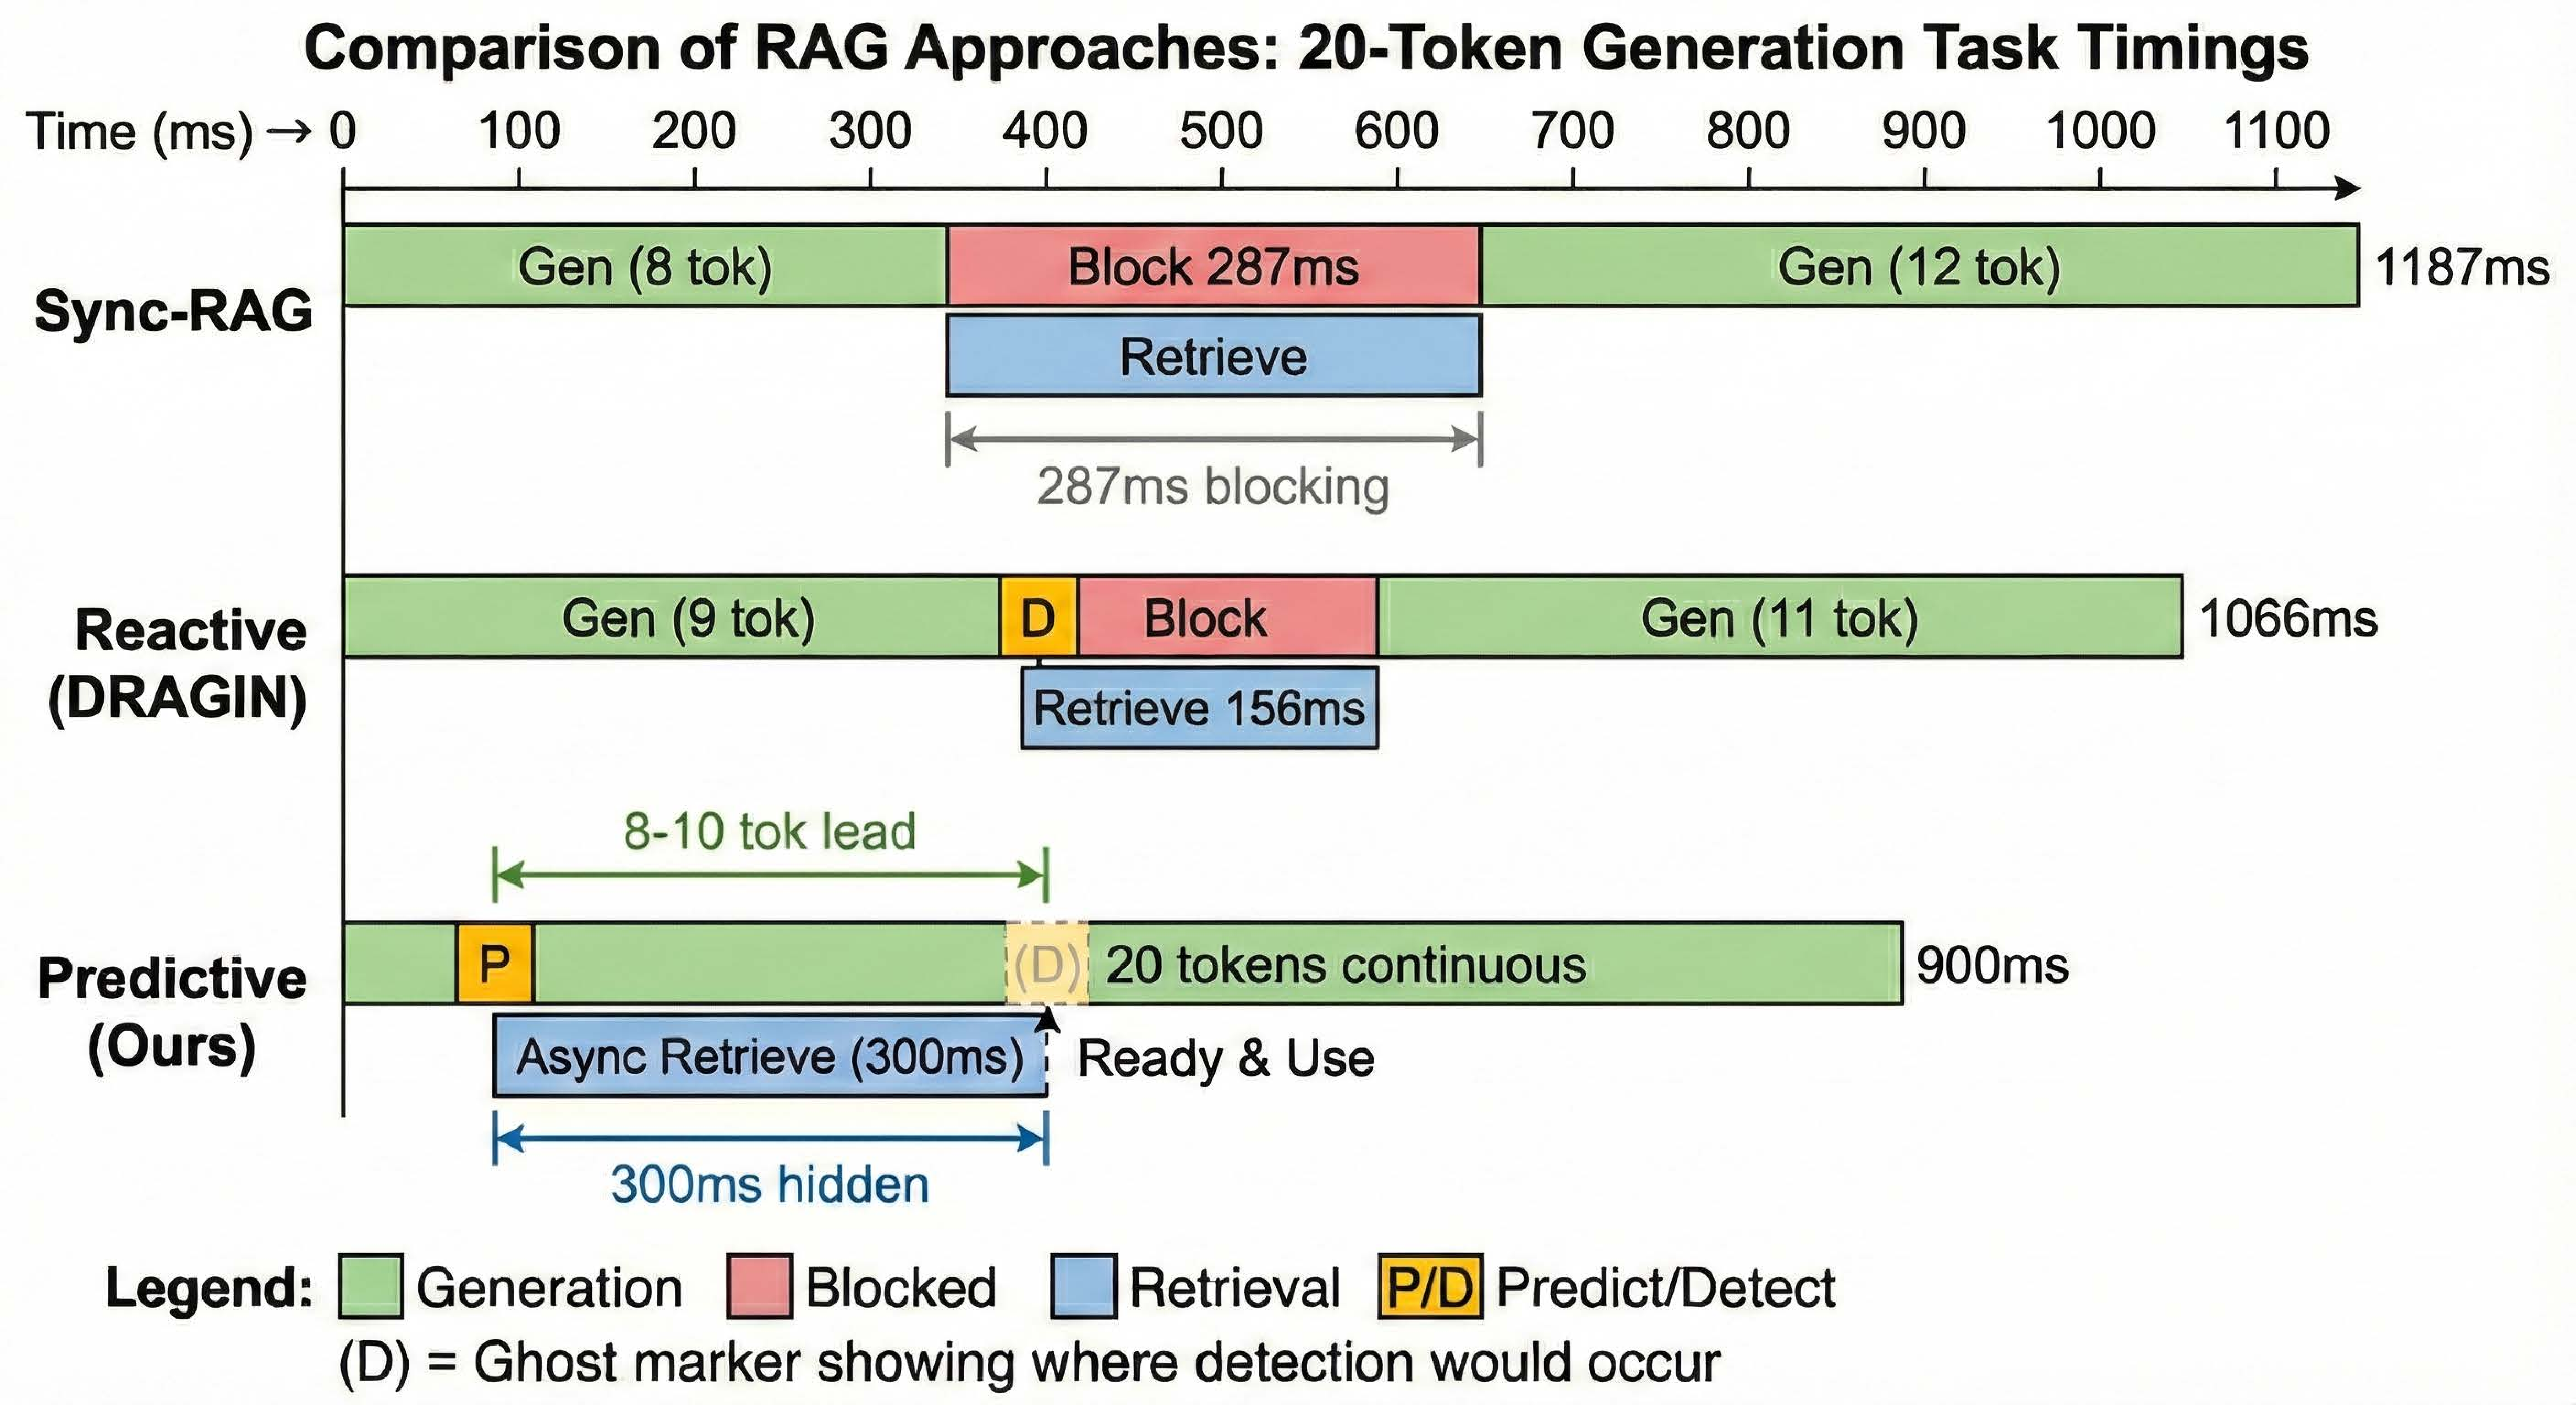
\includegraphics[height=4.7cm]{fig_timeline_comparison.pdf}
  \end{center}
  \note{
    \textbf{(~35s)} RAG fixes hallucination by pulling in external knowledge, but retrieval
    sits on the critical path: 100 to 500 ms per call, and hard queries need many calls.
    The root cause is architectural --- today's RAG is synchronous: when the model gets
    uncertain and triggers retrieval, it simply stops generating and waits, here 287 ms idle.
    So you either allow many retrievals and pay the latency, or cap retrieval and lose
    accuracy. Recent parallel methods run retrieval in the background, but they trigger on
    fixed heuristics and query with stale context --- they hide the clock but fetch the
    wrong thing.
  }
\end{frame}

% ~~~~~~~~~~~~~~~~~~~~~~~~~~~~~~~~~~~~~~~~~~~~~~~~~~~~~~~~~~~~~~~~~~~~~~~~~~~~~~
% 3. KEY INSIGHT
\begin{frame}{Key insight: information needs are foreshadowed}
  \begin{itemize}
    \item Before uncertainty becomes critical, the model's internal state has already shifted: \textbf{entropy trajectories}, \textbf{attention allocation}, and \textbf{value-vector dynamics}.
    \item These precursors appear \emphasize{8--16 tokens early} --- enough lead time to retrieve in the background before generation reaches the gap.
    \item The same signals also indicate \emphasize{what} will be needed, so the query can be built \emphasize{before} the gap appears.
  \end{itemize}
  \vspace{0.35cm}
  \begin{center}
  \begin{tikzpicture}[font=\footnotesize,
      tok/.style={circle, draw=Gray!75, fill=gray!12, minimum size=0.5cm, inner sep=0pt},
      pred/.style={circle, draw=primary, line width=1pt, fill=primary!18, minimum size=0.5cm, inner sep=0pt},
      use/.style={circle, draw=primary, fill=primary, text=white, minimum size=0.5cm, inner sep=0pt, font=\scriptsize\bfseries},
      flow/.style={-{Latex[length=1.4mm]}, draw=Gray!75, line width=0.6pt},
      lbl/.style={text=text, font=\scriptsize, align=center},
      stp/.style={text=primary, font=\scriptsize\bfseries}]
    % --- token stream (generation, never interrupted) ---
    \foreach \i/\x in {1/0, 3/2.6, 4/3.9, 5/5.2, 7/7.8, 8/9.1}{ \node[tok] (t\i) at (\x,0) {}; }
    \node[pred] (t2) at (1.3,0) {};
    \node[use]  (t6) at (6.5,0) {\ding{51}};
    \foreach \i [evaluate=\i as \j using int(\i+1)] in {1,...,7}{ \draw[flow] (t\i) -- (t\j); }
    % --- step 3: overlap (label over the continuous stream) ---
    \node[stp] at (4.55,0.95) {3 \,\textperiodcentered\, Overlap};
    \node[lbl]  at (4.55,0.6)  {generation continues uninterrupted};
    % --- step 1: predict ---
    \node[stp] at (1.3,-0.7) {1 \,\textperiodcentered\, Predict};
    \node[lbl]  at (1.3,-1.04) {signals fire early};
    % --- step 2: prefetch (background retrieval bar under tokens 2--5) ---
    \node[draw=primary, fill=primary!10, rounded corners=2pt, minimum width=4.05cm,
          minimum height=0.5cm, font=\scriptsize, text=text] (bar) at (3.25,-1.75)
          {\textbf{\textcolor{primary}{2 \,\textperiodcentered\, Prefetch}}\, retrieve in background};
    \draw[-{Latex[length=1.4mm]}, primary, dashed, line width=0.6pt]
          (bar.east) -- node[right=0pt, font=\scriptsize, text=primary] {ready} (t6.south);
    % --- lead-time brace from predict to use ---
    \draw[decorate, decoration={brace, amplitude=4pt, mirror}, Gray]
          (1.3,-2.25) -- (6.5,-2.25)
          node[midway, below=4pt, stp] {8--16 token lead time};
  \end{tikzpicture}
  \end{center}
  \note{
    \textbf{(~33s)} Our key observation: the need for retrieval doesn't appear out of nowhere.
    Several tokens before the model gets stuck, its internals already move in a
    characteristic way --- entropy, attention, and the value vectors. We can read those
    signals 8 to 16 tokens ahead. That's the lead time we need to retrieve in the
    background. And crucially, the same signals tell us \emph{what} to look for, so we can
    construct the query before the uncertainty actually arrives. Predict, prefetch the
    aligned content, and overlap it with generation.
  }
\end{frame}

% ~~~~~~~~~~~~~~~~~~~~~~~~~~~~~~~~~~~~~~~~~~~~~~~~~~~~~~~~~~~~~~~~~~~~~~~~~~~~~~
% 4. APPROACH / ARCHITECTURE
\begin{frame}{Approach: decouple retrieval from generation}
  \begin{columns}[T,onlytextwidth]
    \column{0.54\textwidth}
      Three learned components answer three questions:
      \begin{itemize}
        \item \textbf{Retrieval Predictor} --- \emphasize{When} to trigger, from internal signals within a lookahead horizon.
        \item \textbf{Context Monitor} --- \emphasize{Whether} context is sufficient, and how long to wait before querying.
        \item \textbf{Query Generator} --- \emphasize{What} to retrieve, as a context-aware query (T5-small).
      \end{itemize}
      \vspace{0.2cm}
      Retrieval runs asynchronously; results sit in a cache and are used with \emphasize{no added latency}. A synchronous fallback guarantees correctness.
    \column{0.44\textwidth}
      \centering
      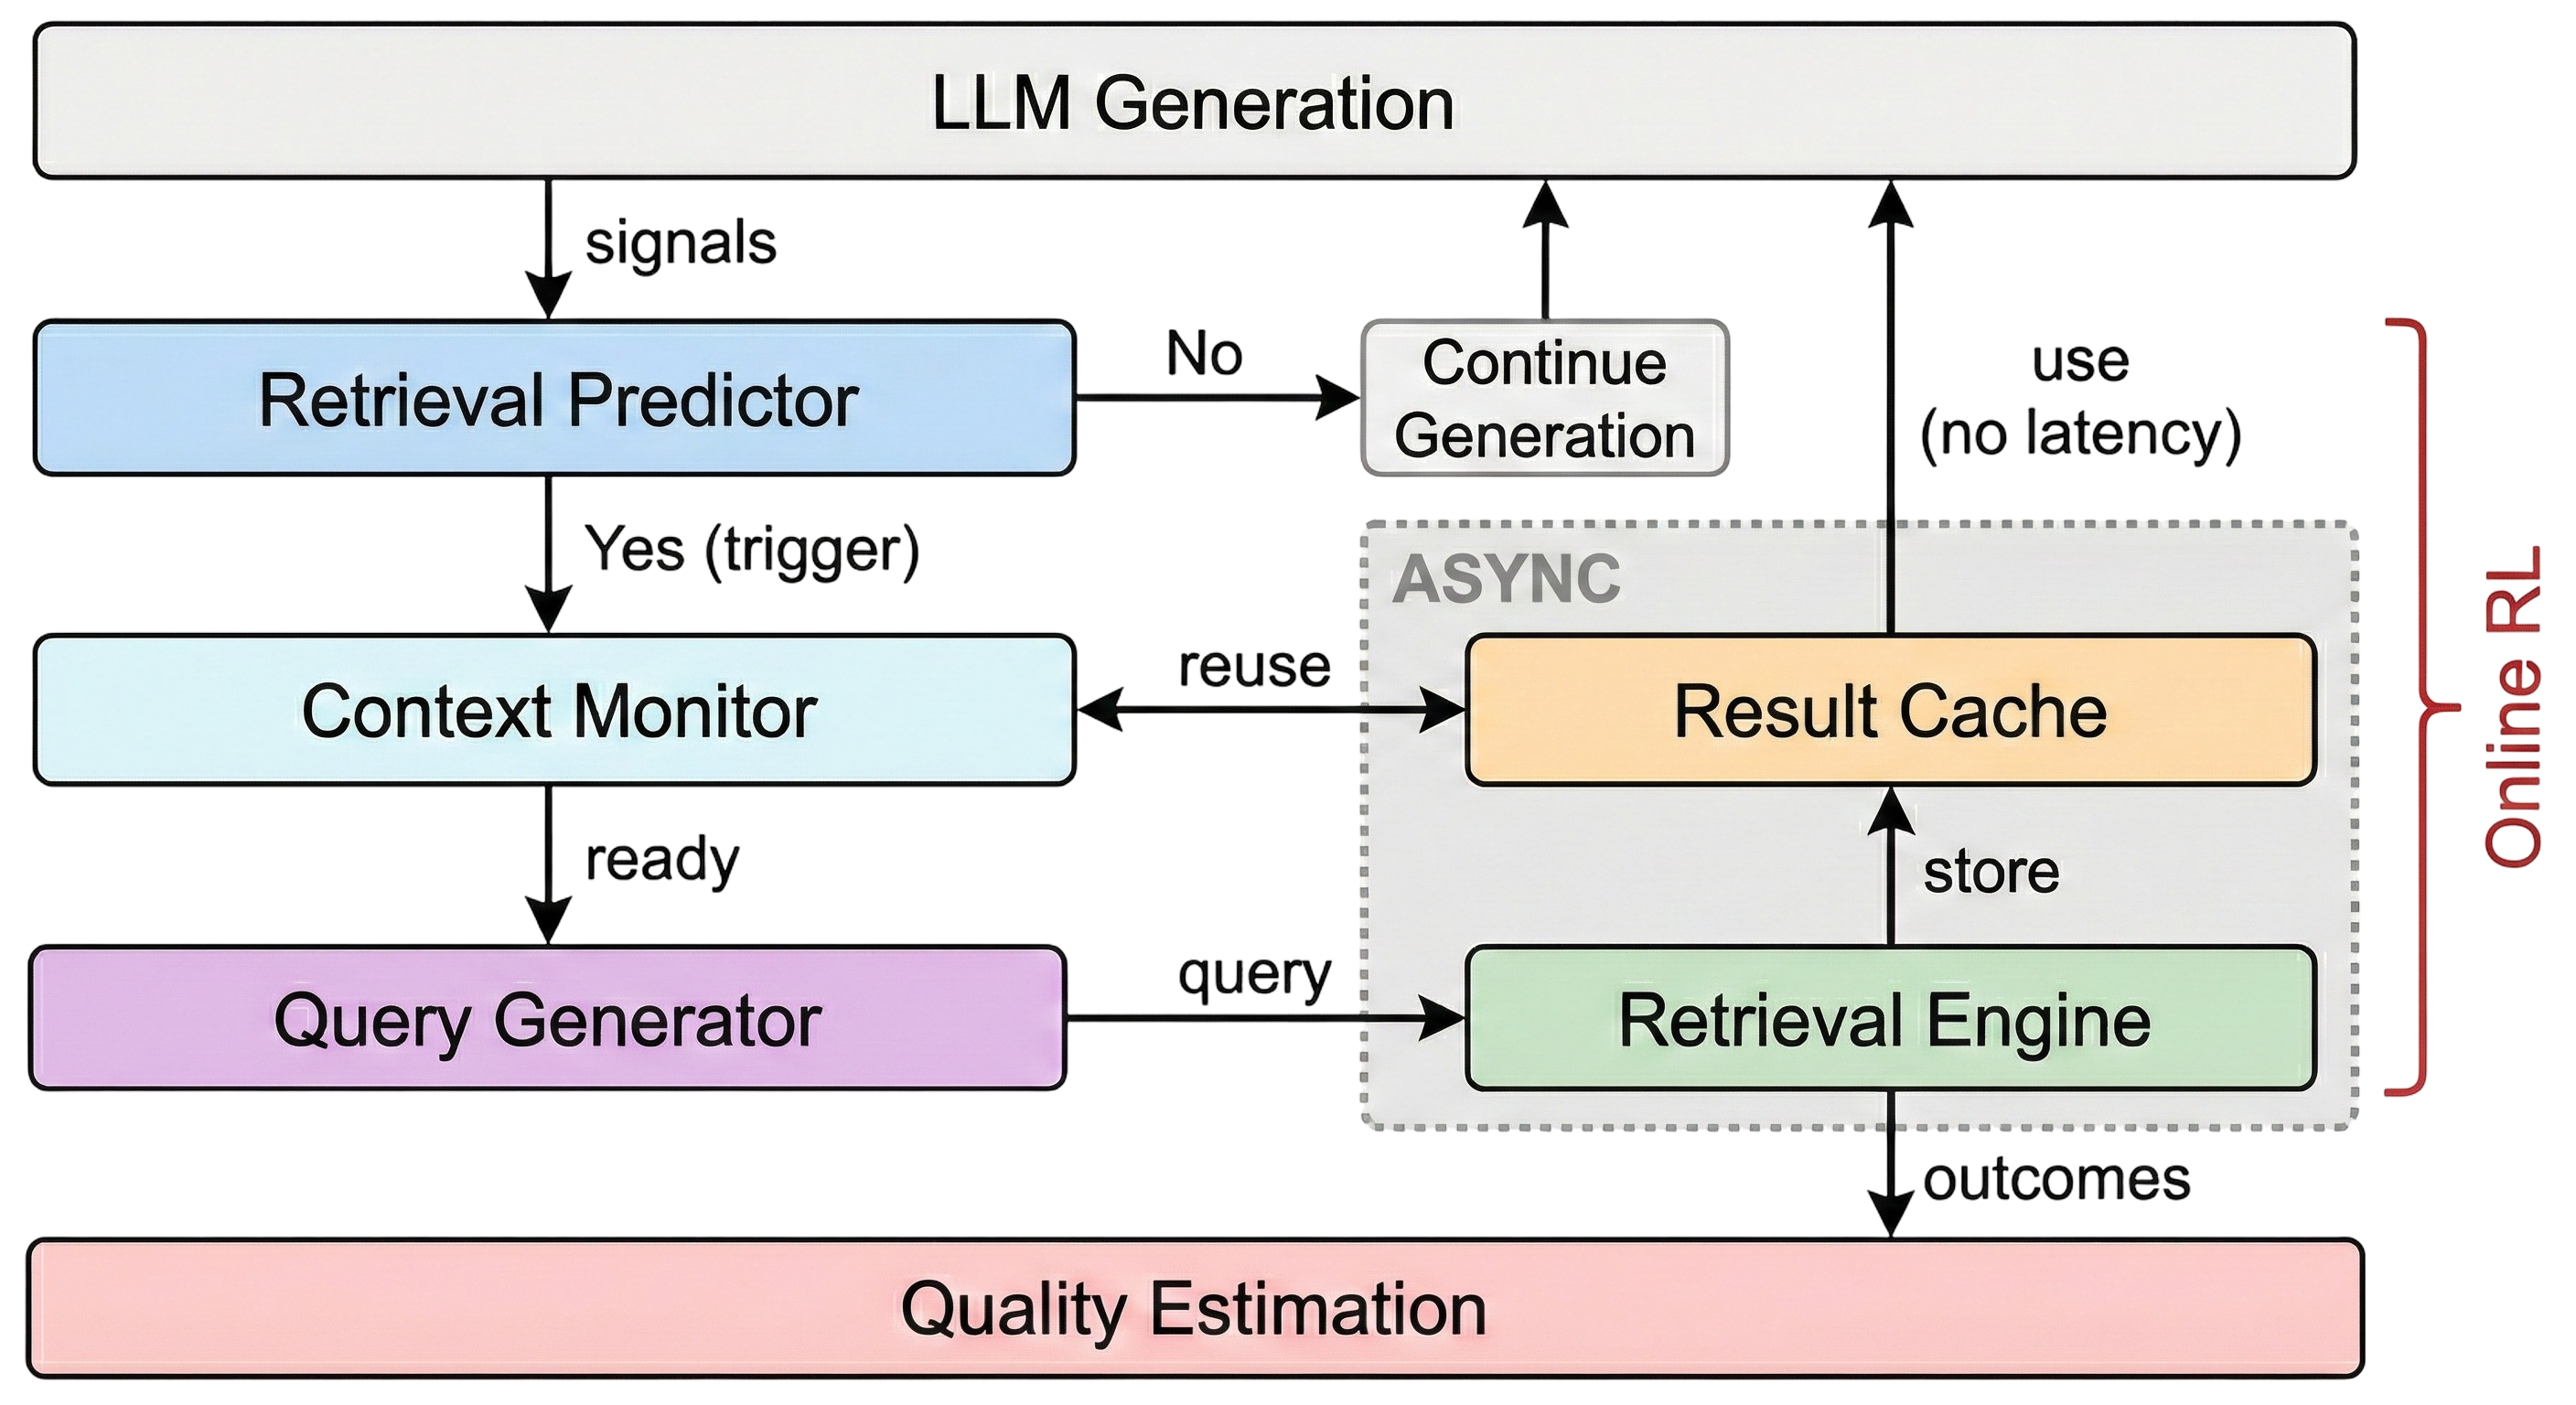
\includegraphics[width=\textwidth]{FigB_VerC.png}
  \end{columns}
  \note{
    \textbf{(~42s)} The framework decouples retrieval from generation with three small
    learned components, each answering one question. The Retrieval Predictor decides
    \emph{when} to trigger, reading the internal signals within a lookahead window. The
    Context Monitor decides \emph{whether} we have enough context yet, and how many tokens
    to wait so the query isn't half-formed. The Query Generator decides \emph{what} to
    fetch --- a context-aware query from a small T5. Retrieval then runs asynchronously;
    documents land in a result cache and are consumed with no added latency. If a
    prediction misses, we fall back to synchronous retrieval, so correctness is never at
    risk.
  }
\end{frame}

% ~~~~~~~~~~~~~~~~~~~~~~~~~~~~~~~~~~~~~~~~~~~~~~~~~~~~~~~~~~~~~~~~~~~~~~~~~~~~~~
% 5. LEARNING
\begin{frame}{Learning: pretrain once, then adapt online}
  \begin{itemize}
    \item \textbf{Multi-task pretraining} on generation traces with \emphasize{automatic oracle labels} --- no manual annotation.
    \item \textbf{Online adaptation} via policy gradient with \emphasize{action-specific feedback} (a contextual-bandit structure --- dense, per-decision reward).
    \item A gated cascade of four actions --- \textbf{Generate / Reuse / Accumulate / Fetch} --- where each action's reward updates \emphasize{only} the component that made it.
    \item Total cost: \emphasize{+62M} parameters over an 8B model and \emphasize{+2.7\,ms} per token.
  \end{itemize}
  \note{
    \textbf{(~28s)} All three components are pretrained jointly. Labels come automatically
    from generation traces --- we compare answers with and without retrieval --- so there's
    no hand annotation. After deployment, the system keeps adapting with a policy gradient.
    Because each decision gets immediate, action-specific feedback, it's a contextual bandit,
    not long-horizon RL --- the reward for Generate, Reuse, Accumulate, or Fetch updates only
    the component responsible. The whole stack is 62 million parameters on top of an 8B model
    and adds under 3 ms per token.
  }
\end{frame}

% ~~~~~~~~~~~~~~~~~~~~~~~~~~~~~~~~~~~~~~~~~~~~~~~~~~~~~~~~~~~~~~~~~~~~~~~~~~~~~~
% 6. MAIN RESULTS
\begin{frame}{Results: latency down, quality held}
  \begin{center}
    \setlength{\extrarowheight}{2pt}
    \begin{tabular}{lcccc}
      \toprule
      \textbf{Method} & \textbf{EM} & \textbf{TTFT} & \textbf{E2E} & \textbf{Ret/1K} \\
      \midrule
      No retrieval        & 32.8 & 42\,ms  & 2.3\,s & 0 \\
      Sync-RAG            & 69.2 & 287\,ms & 9.2\,s & 86 \\
      PipeRAG (async)     & 66.8 & 118\,ms & 5.6\,s & 67 \\
      \rowcolor{primary!10}\textbf{Ours (predictive)} & \textbf{68.7} & \textbf{108\,ms} & \textbf{5.2\,s} & \textbf{59} \\
      \bottomrule
    \end{tabular}
  \end{center}
  \vspace{0.15cm}
  {\small Llama-3.1-8B, four QA benchmarks (HotpotQA shown). TTFT: time-to-first-token; E2E: end-to-end latency; Ret/1K: retrievals per 1{,}000 tokens.}
  \begin{itemize}
    \item \emphasize{$-$62.4\%} time-to-first-token, \emphasize{$-$43.5\%} end-to-end latency, \emphasize{31\%} fewer retrievals.
    \item Answer quality within \emphasize{1\%} of synchronous RAG --- and better on \emph{both} quality and efficiency than prior async (PipeRAG).
  \end{itemize}
  \note{
    \textbf{(~35s)} Here is the headline. Synchronous RAG is accurate but slow --- 287 ms to
    first token, 9.2 seconds end to end. We cut time-to-first-token by 62\%, end-to-end
    latency by 43\%, and use about a third fewer retrievals --- while keeping exact-match
    within one point of synchronous RAG. Against the strongest prior async method, PipeRAG,
    we are better on both axes at once: higher quality and lower latency, because we fetch
    aligned content instead of stale content.
  }
\end{frame}

% ~~~~~~~~~~~~~~~~~~~~~~~~~~~~~~~~~~~~~~~~~~~~~~~~~~~~~~~~~~~~~~~~~~~~~~~~~~~~~~
% 7. PREDICTION QUALITY
\begin{frame}{Why it works: accurate, well-timed prediction}
  \begin{columns}[c,onlytextwidth]
    \column{0.5\textwidth}
      \centering
      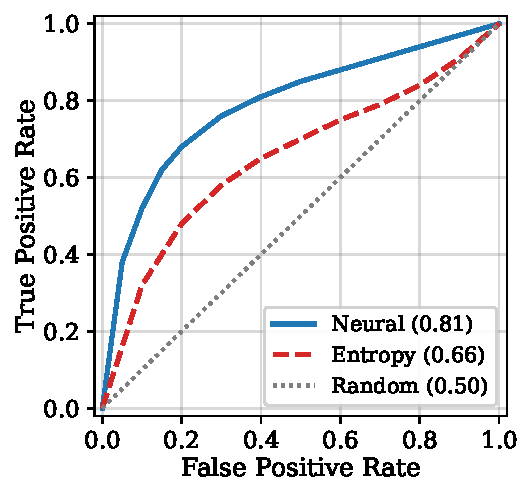
\includegraphics[height=3.6cm]{fig_roc_curves.pdf}\\
      {\small Prediction accuracy}
    \column{0.5\textwidth}
      \centering
      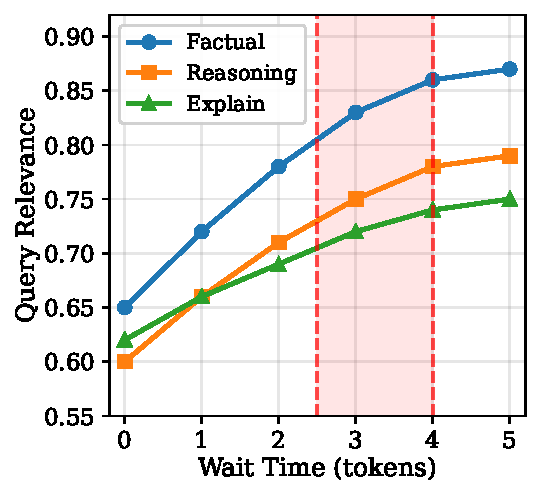
\includegraphics[height=3.6cm]{fig_query_relevance.pdf}\\
      {\small Query relevance vs. wait time}
  \end{columns}
  \vspace{0.25cm}
  \begin{itemize}
    \item Predictor reaches \emphasize{AUROC 0.81} vs.\ 0.66 for entropy alone --- a 23\% gain in identifying upcoming needs.
    \item High-confidence predictions give \emphasize{8.7 tokens} of lead --- over 400\,ms for retrieval to complete.
    \item Waiting just \emphasize{3--4 tokens} raises query relevance by up to \emphasize{23\%}.
  \end{itemize}
  \note{
    \textbf{(~33s)} Two things make this work. Left: the learned predictor reaches an AUROC
    of 0.81, versus 0.66 if you just threshold the current entropy --- a 23\% improvement at
    spotting needs before they arrive. And high-confidence predictions give us about 8.7
    tokens of lead time, which is over 400 ms --- enough to finish a retrieval. Right: the
    Context Monitor's adaptive waiting matters --- pausing just 3 to 4 tokens lets a partial
    phrase complete and lifts query relevance by up to 23\%.
  }
\end{frame}

% ~~~~~~~~~~~~~~~~~~~~~~~~~~~~~~~~~~~~~~~~~~~~~~~~~~~~~~~~~~~~~~~~~~~~~~~~~~~~~~
% 8. ROBUSTNESS / GENERALITY
\begin{frame}{It holds up across settings}
  \begin{columns}[c,onlytextwidth]
    \column{0.46\textwidth}
      \centering
      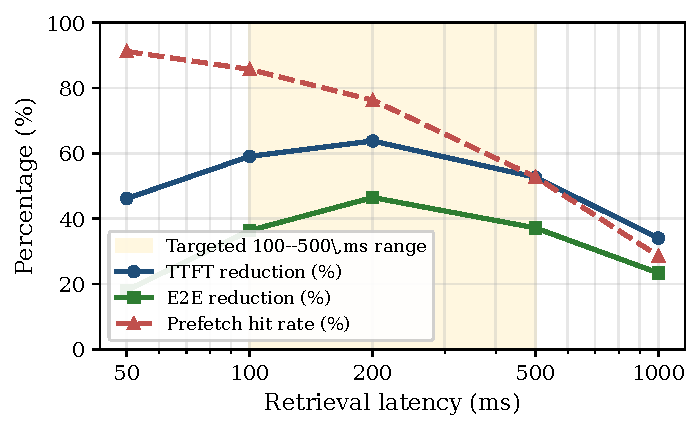
\includegraphics[width=\textwidth]{fig_latency_sweep.pdf}\\
      {\small Gains vs.\ retrieval latency}
    \column{0.54\textwidth}
      \begin{itemize}
        \item Gains peak near \emphasize{200\,ms} and \emphasize{degrade gracefully}; the synchronous fallback always floors at the baseline.
        \item Consistent across \emphasize{six models} (Llama, GPT-OSS, Qwen): TTFT $-$61.5\% to $-$63.4\%.
        \item Also improves \textbf{code completion} and \textbf{summarization}.
        \item Tail latency stays bounded: miss-query P99 (14.0\,s) $<$ Sync-RAG P95 (15.2\,s).
      \end{itemize}
  \end{columns}
  \note{
    \textbf{(~27s)} It generalizes. Sweeping retrieval latency, the benefit peaks around
    200 ms and falls off gracefully --- and because of the synchronous fallback, the worst
    case is never worse than the baseline. The same thresholds drive six different models,
    Llama, GPT-OSS, and Qwen, with 61 to 63\% faster first token, and the method also helps
    code completion and summarization. Even the tail is controlled: a missed prediction's
    P99 still beats synchronous RAG's P95.
  }
\end{frame}

% ~~~~~~~~~~~~~~~~~~~~~~~~~~~~~~~~~~~~~~~~~~~~~~~~~~~~~~~~~~~~~~~~~~~~~~~~~~~~~~
% 9. TAKEAWAY
\begin{frame}{Takeaway}
  \begin{itemize}
    \item Retrieval needs are \emphasize{predictable} from generation dynamics --- several tokens in advance.
    \item Deciding \emphasize{when}, \emphasize{whether}, and \emphasize{what} to retrieve hides latency \emphasize{without} sacrificing relevance.
    \item \emphasize{$-$43.5\%} end-to-end latency, \emphasize{$-$62.4\%} time-to-first-token, quality within \emphasize{1\%} of synchronous RAG.
  \end{itemize}
  \vfill
  \begin{columns}[c,onlytextwidth]
    \column{0.7\textwidth}
      \textbf{Wuyang Zhang} \quad \textbf{Shichao Pei}\\
      University of Massachusetts Boston\\
      {\small\texttt{shichao.pei@umb.edu}}
    \column{0.3\textwidth}
      \hfill
\includegraphics[height=1.2cm]{Blue-UMB-logo-lockup.png}
  \end{columns}
  \vspace{0.4cm}
  \begin{center}
    \emphasize{\textbf{Thank you.}}
  \end{center}
  \vfill
  \note{
    \textbf{(~18s)} To wrap up: the need for retrieval is predictable from the model's own
    generation dynamics, several tokens ahead. By learning when, whether, and what to
    retrieve, we hide retrieval latency without giving up relevance --- 43\% lower
    end-to-end latency, 62\% faster first token, and quality within one point of synchronous
    RAG. Thank you; happy to take questions.
  }
\end{frame}

\end{document}
